\chapter{Work/Design}

In this chapter I will describe the work I have done in order to implement model-based testing into the MCP. The workload that is contained in the implementation and description herein includes implementation of a monadic parser that reads the xml-specification files, an update of the fields and contents of fields in the xml-specification files, as well as a model, that is built upon the foundation of aforementioned updated xml-specification. %TODO Hvis det fungerer med interpreter(parser(xml))=model, så skriv det på.

\section{Updated Data}

As discussed in Section \ref{sec:Data}, in order to create uniform models, upon which to execute tests, the structure of the xml-specification files needs to be altered in a manner that adds uniformity to the xml-specification files. 

One way to implement these changes is make the user able to assign variables, based on a fixed collection of available options. An example of execution of this is given in Figure \ref{fig:entityStruct}. Each level in the tree describes a field, which can be filled with predefined variables, which in the end forms a clear and unambiguous collection of entities, along with a similarly unambiguous description of relations, exchange-patterns, and security precautions. 
% Hvordan ville JEG designe en specifikation
% What data WILL be available after?
\begin{figure}
	\centering
	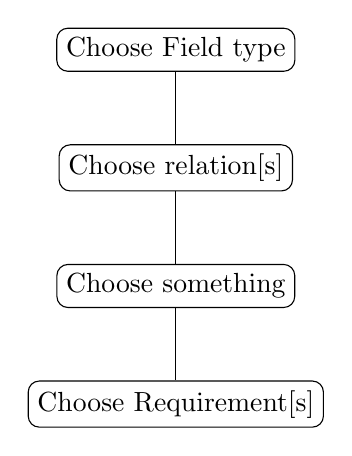
\begin{tikzpicture}[sibling distance=10em,
		every node/.style = {shape=rectangle, rounded corners,
			draw, align=center}]]
		\node {Choose Field type}
			child{
				node{Choose relation[s]}
				child{
					node{Choose something}
					child{
						node{Choose Requirement[s]} %requirement[s] to above specific relatino
					}
				}
			};
	\end{tikzpicture}
	\caption{New entity structure in xml-specification files.}
	\label{fig:entityStruct}
\end{figure}

The updated xml-specification files would be limiting the flexibility of the models in some aspects, as not all maritime services would follow the layout given in Figure \ref{fig:entityStruct}, however the example given is the earliest version of the domain-specific language. Following complex structures of various maritime services, the domain-specific language of the specification files can scale in complexity with the requirements set up by the maritime services.

\section{Parser Grammars}

\subsection{ServiceInstanceSchema}		%EFTERFØLGENDE grammatik -- den opdaterede, som man godt kan få noget ud af
\subsection{General Grammar}			%EFTERFØLGENDE grammatik -- den opdaterede, som man godt kan få noget ud af

\section{Implementation in the MCP}

% Monadisk parsing

% Evt. lav en specifikationsXML selv.

% Evt lav nedenstående til et Chapter

\section{Technical Implementation}
\subsection{Executing Instructions}

\section{Testing}


